\documentclass{article}

\usepackage{fontspec}
\usepackage{fullpage}
\usepackage{multicol}
\usepackage{multirow}
\usepackage{tikz}

\begin{document}

\newfontfamily\swfill{SuttonSignWritingFill.ttf}
\newfontfamily\swline{SuttonSignWritingLine.ttf}
\newcommand{\bul}{\hfil$\bullet$&}
\renewenvironment{glossary}{\begin{multicols}{5}\begin{center}}{\end{center}\end{multicols}}
\setcounter{secnumdepth}{0}
\setlength{\columnseprule}{1pt}

\section{Supplement For Lesson 11}

\begin{center}
\it
Objectives inspired by, vocabulary transcribed from, and sentences and story by Bill Vicars.

Handshape photos by Adam Frost.

No endorsement implied nor given by either.
\end{center}

\subsection{Objectives}

\begin{tabular}{p{1cm}p{14cm}}
\bul I have completed the objectives for this lesson.\\
\bul I know which base symbols are in Symbol Groups timing and head.\\
\bul I am able to read, write, and sign the ASL handshapes in symbol group six.\\
\bul I am able to recognize the vocabulary for this lesson.\\
\bul I am able to read the practice sentences for this lesson.\\
\bul I am able to read the practice story for this lesson.\\
\end{tabular}

\subsection{Symbol Groups Timing and Head}

The twenty-first Symbol Group we informally call timing, though it's official name is ``Dynamics \& Timing''.

\begin{center}
\begin{tabular}{rcrc}
\textbf{Base Symbol}&\textbf{Example}&\textbf{Base Symbol}&\textbf{Example}\\
Fast            &B506x504S2f700494x497&Slow                 &B519x506S2f800481x495\\
Tense           &B506x503S2f900495x498&Relaxed              &B506x504S2fa00495x497\\
Same Time       &B508x503S2fb00493x497&Same Time Alternating&B508x506S2fc00493x495\\
Every Other Time&B512x503S2fd00489x497&Gradual              &B508x507S2fe00493x493\\
\end{tabular}
\end{center}

The twenty-second Symbol Group we informally call head, though it's official name is also ``Head''.

\begin{center}
\begin{tabular}{rcrc}
\textbf{Base Symbol}&\textbf{Example}&\textbf{Base Symbol}&\textbf{Example}\\
Head                                             &B518x518S2ff00482x483&Head Rims                                &B518x518S30000482x483\\
Head Movement Straight Wall Plane                &B518x523S30100482x477&Head Movement Tilts Wall Plane           &B518x523S30200482x478\\
Head Movement Straight Floor Plane               &B518x523S30300482x477&Head Movement Curves Wall Plane          &B518x522S30400482x478\\
Head Movement Curves Floor Plane                 &B518x521S30500482x479&Head Movement Circles                    &B518x519S30600482x481\\
Face Direction Positions, Nose Forward Tilting   &B518x518S30700482x483&Face Direction Positions, Nose Up or Down&B518x522S30800482x478\\
Face Direction Positions, Nose Up or Down Tilting&B518x522S30900482x479\\
\end{tabular}
\end{center}

Before you can consider this lesson complete, you need to be able to list off the symbol grops as:
``one, two, three, four, five, six, seven, eight, nine, thumb;''
``contact, finger, wall, diagonal, floor, curve wall, hit wall, hit floor, curve floor, circle;''
``timing, head.''

Don't forget that we consider the groups as being in three sets of ten so there is also a semicolon after circle.

Category three is dynamics, and the solitary base symbol gets is timing.
Category four is face and it gets half of the third group \emph{generally} moving from top to bottom.

\subsection{Remaining ASL Handshapes From Symbol Group Six}

The eleven handshapes in Symbol Group Six used by ASL in order are:
Index Middle Ring;
Index Middle Ring on Circle;
Index Middle Ring, Bent;
Index Middle Ring, Unit;
Index Middle Ring, Unit Hinge;
Baby Up;
{\bf
Baby Thumb;
Baby Thumb on Hinge;
Baby Index Thumb;
Baby Index Thumb on Hinge;
and Baby Index.
}

\subsubsection{The Baby Thumb Handshape}

\begin{center}
\begin{tabular}{r*{6}{c}}
&\textbf{Fill 1}&\textbf{Fill 2}&\textbf{Fill 3}&\textbf{Fill 4}&\textbf{Fill 5}&\textbf{Fill 6}\\
\multirow{2}{*}{\textbf{Right}}&
B514x510S19a00486x490&
B514x510S19a10486x490&
B514x510S19a20486x490&
B514x510S19a30486x490&
B514x510S19a40486x490&
B514x510S19a50486x490\\
&
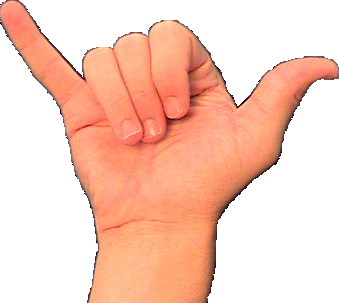
\includegraphics[scale=0.1]{images/06-07-1.jpg}&
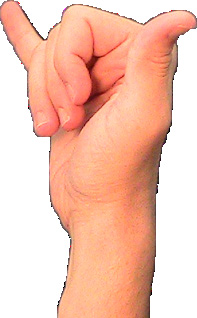
\includegraphics[scale=0.1]{images/06-07-2.jpg}&
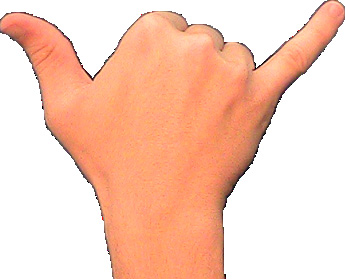
\includegraphics[scale=0.1]{images/06-07-3.jpg}&
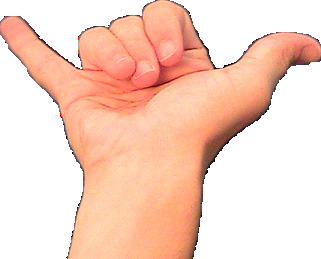
\includegraphics[scale=0.1]{images/06-07-4.jpg}&
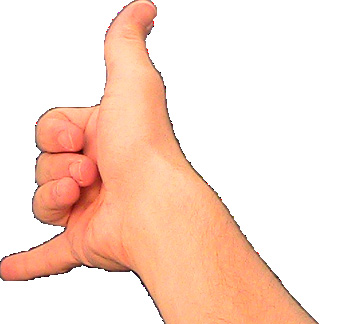
\includegraphics[scale=0.1]{images/06-07-5.jpg}&
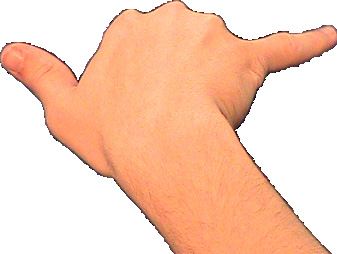
\includegraphics[scale=0.1]{images/06-07-6.jpg}\\
\textbf{Left}&
B514x510S19a08486x490&
B514x510S19a18486x490&
B514x510S19a28486x490&
B514x510S19a38486x490&
B514x510S19a48486x490&
B514x510S19a58486x490\\
\end{tabular}
\end{center}

\subsubsection{The Baby Thumb on Hinge Handshape}

\begin{center}
\begin{tabular}{r*{6}{c}}
&\textbf{Fill 1}&\textbf{Fill 2}&\textbf{Fill 3}&\textbf{Fill 4}&\textbf{Fill 5}&\textbf{Fill 6}\\
\multirow{2}{*}{\textbf{Right}}&
B515x511S19b00485x489&
B515x511S19b10485x489&
B515x511S19b20485x489&
B515x511S19b30485x489&
B515x511S19b40485x489&
B515x511S19b50485x489\\
&
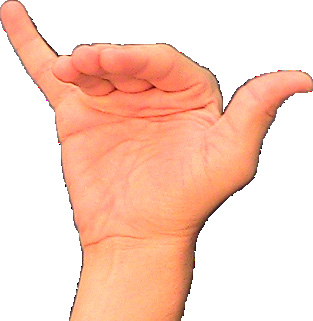
\includegraphics[scale=0.1]{images/06-08-1.jpg}&
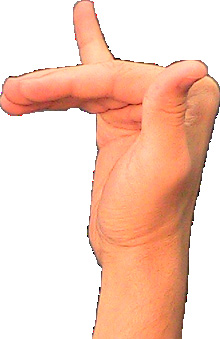
\includegraphics[scale=0.1]{images/06-08-2.jpg}&
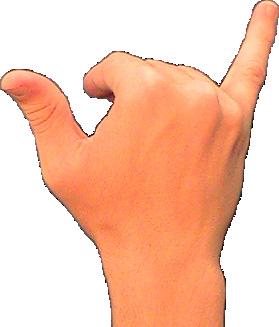
\includegraphics[scale=0.1]{images/06-08-3.jpg}&
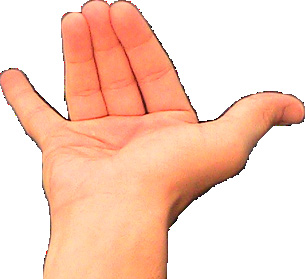
\includegraphics[scale=0.1]{images/06-08-4.jpg}&
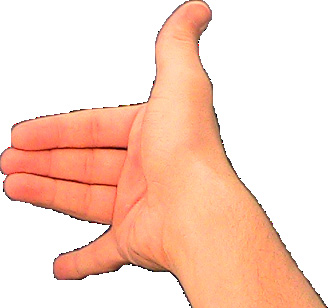
\includegraphics[scale=0.1]{images/06-08-5.jpg}&
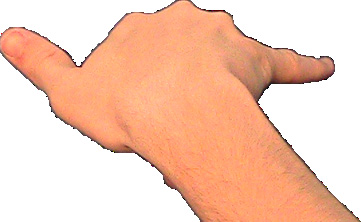
\includegraphics[scale=0.1]{images/06-08-6.jpg}\\
\textbf{Left}&
B515x511S19b08485x489&
B515x511S19b18485x489&
B515x511S19b28485x489&
B515x511S19b38485x489&
B515x511S19b48485x489&
B515x511S19b58485x489\\
\end{tabular}
\end{center}

\subsubsection{The Baby Index Thumb Handshape}

\begin{center}
\begin{tabular}{r*{6}{c}}
&\textbf{Fill 1}&\textbf{Fill 2}&\textbf{Fill 3}&\textbf{Fill 4}&\textbf{Fill 5}&\textbf{Fill 6}\\
\multirow{2}{*}{\textbf{Right}}&
B514x515S19c00486x486&
B514x515S19c10486x486&
B514x515S19c20486x486&
B514x515S19c30486x486&
B514x515S19c40486x486&
B514x515S19c50486x486\\
&
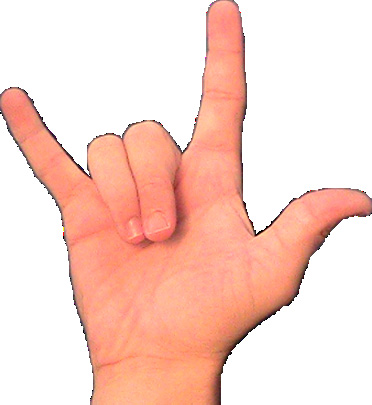
\includegraphics[scale=0.1]{images/06-09-1.jpg}&
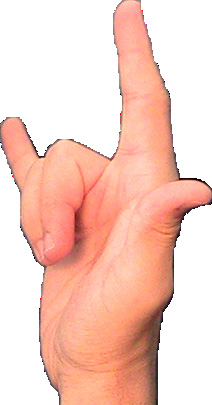
\includegraphics[scale=0.1]{images/06-09-2.jpg}&
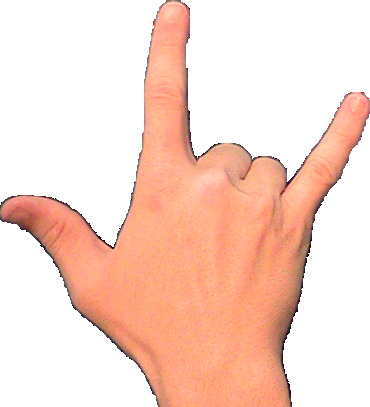
\includegraphics[scale=0.1]{images/06-09-3.jpg}&
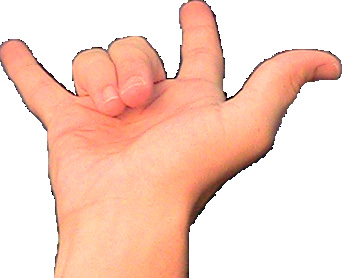
\includegraphics[scale=0.1]{images/06-09-4.jpg}&
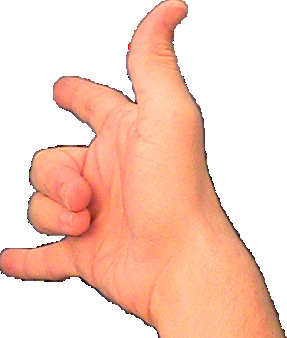
\includegraphics[scale=0.1]{images/06-09-5.jpg}&
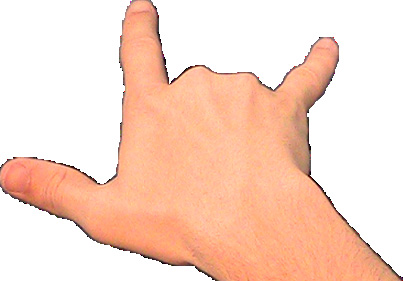
\includegraphics[scale=0.1]{images/06-09-6.jpg}\\
\textbf{Left}&
B514x515S19c08486x486&
B514x515S19c18486x486&
B514x515S19c28486x486&
B514x515S19c38486x486&
B514x515S19c48486x486&
B514x515S19c58486x486\\
\end{tabular}
\end{center}

\subsubsection{The Baby Index Thumb on Hinge Handshape}

\begin{center}
\begin{tabular}{r*{6}{c}}
&\textbf{Fill 1}&\textbf{Fill 2}&\textbf{Fill 3}&\textbf{Fill 4}&\textbf{Fill 5}&\textbf{Fill 6}\\
\multirow{2}{*}{\textbf{Right}}&
B515x515S19d00486x486&
B515x515S19d10486x486&
B515x515S19d20486x486&
B515x515S19d30486x486&
B515x515S19d40486x486&
B515x515S19d50486x486\\
&
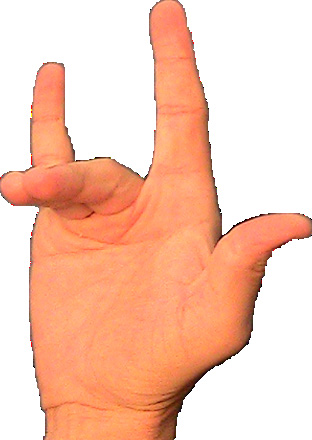
\includegraphics[scale=0.1]{images/06-10-1.jpg}&
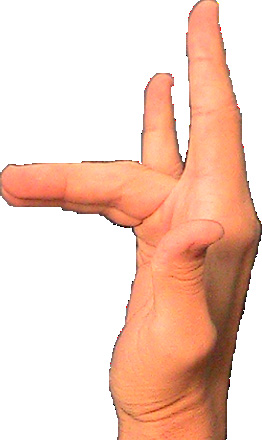
\includegraphics[scale=0.1]{images/06-10-2.jpg}&
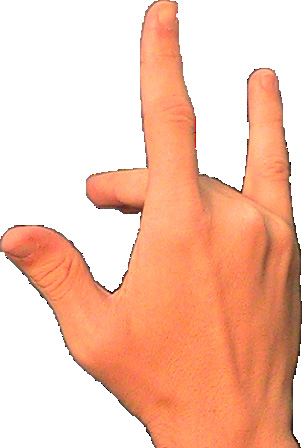
\includegraphics[scale=0.1]{images/06-10-3.jpg}&
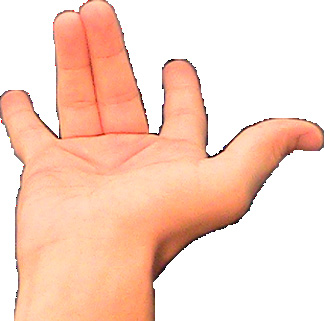
\includegraphics[scale=0.1]{images/06-10-4.jpg}&
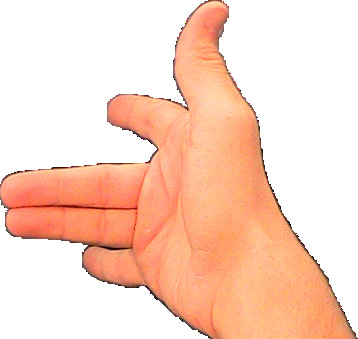
\includegraphics[scale=0.1]{images/06-10-5.jpg}&
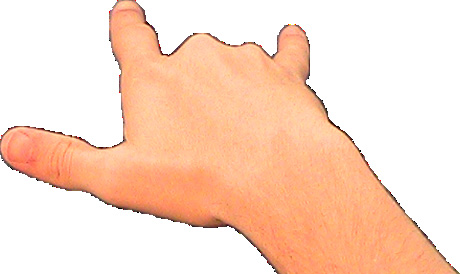
\includegraphics[scale=0.1]{images/06-10-6.jpg}\\
\textbf{Left}&
B515x515S19d08486x486&
B515x515S19d18486x486&
B515x515S19d28486x486&
B515x515S19d38486x486&
B515x515S19d48486x486&
B515x515S19d58486x486\\
\end{tabular}
\end{center}

\subsubsection{The Baby Index handshape}

\begin{center}
\begin{tabular}{r*{6}{c}}
&\textbf{Fill 1}&\textbf{Fill 2}&\textbf{Fill 3}&\textbf{Fill 4}&\textbf{Fill 5}&\textbf{Fill 6}\\
\multirow{2}{*}{\textbf{Right}}&
B510x515S1a000490x486&
B510x515S1a010490x486&
B510x515S1a020490x486&
B510x515S1a030490x486&
B510x515S1a040490x486&
B510x515S1a050490x486\\
&
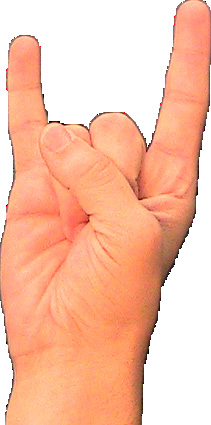
\includegraphics[scale=0.1]{images/06-11-1.jpg}&
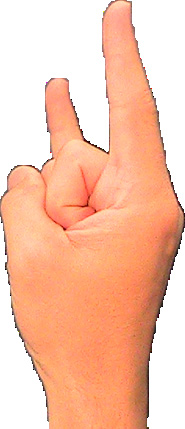
\includegraphics[scale=0.1]{images/06-11-2.jpg}&
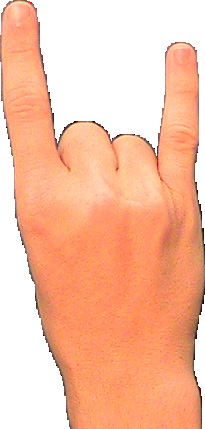
\includegraphics[scale=0.1]{images/06-11-3.jpg}&
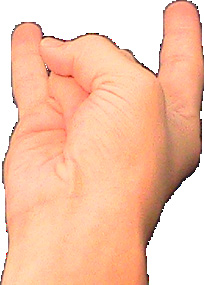
\includegraphics[scale=0.1]{images/06-11-4.jpg}&
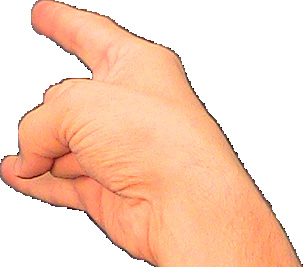
\includegraphics[scale=0.1]{images/06-11-5.jpg}&
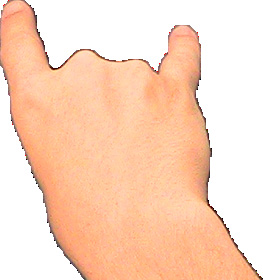
\includegraphics[scale=0.1]{images/06-11-6.jpg}\\
\textbf{Left}&
B510x515S1a008490x486&
B510x515S1a018490x486&
B510x515S1a028490x486&
B510x515S1a038490x486&
B510x515S1a048490x486&
B510x515S1a058490x486\\
\end{tabular}
\end{center}

\subsection{Vocabulary}

\begin{glossary}

\textbf{about}\\
AS10012S10019S2ef00S20500M527x528S10019474x498S10012497x497S2ef00503x472S20500488x483

\textbf{always}\\
AS10000S2e732M513x526S10000493x475S2e732488x510

\textbf{any}
AS1f510S2a204M522x514S1f510479x496S2a204499x486

\textbf{back}\\
AS14720S26707S16d20S14020M526x534S14720475x510S14020497x466S16d20490x494S26707494x503

\textbf{but}\\
AS10021S10029S26506S26512M526x521S10021496x500S10029475x500S26506507x480S26512475x480

\textbf{call}\\
AS19a02S26503S34400M550x522S34400482x483S19a02515x494S26503537x486

\textbf{can't}\\
AS10012S1001aS20e00S22a04M528x523S10012498x478S1001a473x486S20e00500x493S22a04500x508

\textbf{chat}\\
AS14c17S14c1fS23004S23014S2fb04M534x530S14c17507x471S14c1f466x470S23004505x503S23014471x502S2fb04494x524

\textbf{different}\\
AS10021S10029S26506S26512M547x511S10021495x490S10029475x490S26506532x494S26512453x494

\textbf{for}\\
AS10001S20500S30007S26500S10021M551x518S30007482x483S10001523x487S10021521x435S20500508x475S26500535x464

\textbf{great}\\
AS14c20S14c28S26a00S26a10S2fb00M532x527S14c20504x496S14c28469x496S26a00505x482S26a10469x482S2fb00490x473

\textbf{little}\\
AS1dc40S1dc48S26a02S26a16S2fb04M531x533S1dc40507x468S1dc48469x468S26a02506x506S26a16479x506

\textbf{little bit}\\
AS1ea30S21d00M514x516S1ea30491x495S21d00487x484

\textbf{make}\\
AS20310S20314S20500S20300S20300S20500M519x543S20314481x476S20310486x457S20300492x509S20300487x528S20500501x475S20500509x525

\textbf{never}\\
AS15a50S24103S15a40M524x533S15a50476x468S15a40477x506S24103492x482

\textbf{new}\\
AS1821dS15a16S20e00S2880fM532x517S15a16505x505S2880f468x484S20e00491x495S1821d503x492

\textbf{oh I see}\\
AS19a57S23004S36d00M558x523S19a57531x477S23004529x505S36d00479x482

\textbf{or}\\
AS17620S11a20M518x515S11a20503x485S17620483x499

\textbf{people}\\
AS14020S14028S2e700S2e74cM529x537S2e74c474x512S2e700514x497S14020498x463S14028471x478

\textbf{sometimes}\\
AS10041S15a39S20e00S2ea00M528x521S15a39473x479S10041482x491S20e00497x490S2ea00513x483

\textbf{talk}\\
AS14410S20600S33b00M518x541S14410491x510S33b00482x483S20600468x517

\textbf{talk with}\\
AS14447S1444fS22f04S22f14S2fb04M550x526S14447522x475S1444f450x475S22f14458x510S22f04518x511S2fb04491x520

\textbf{thing}\\
AS15a30S26706S22f04M521x527S15a30480x473S26706479x498S22f04479x513

\textbf{tty call}\\
AS10049S10a51S20e00S26607M528x529S10049485x499S10a51495x487S26607485x472S20e00473x494

\textbf{wonderful}\\
AS14c20S14c28S26a00S26a10S2fb00M532x527S14c20504x496S14c28469x496S26a00505x482S26a10469x482S2fb00490x473

\end{glossary}

\subsection{Practice Sheet 11.A}

\begin{multicols}{5}
\begin{center}

M508x515S10000493x485 % 1
M536x504S38800464x496 % .
M518x572S33b00482x483S20500508x516S10000488x512S28e04461x536 % tell me
M527x528S10019474x498S10012497x497S2ef00503x472S20500488x483 % about
M507x523S15a28494x496S26500493x477 % your
M546x575S2ff00482x483S18510521x490S18518452x493S26500525x468S26510458x469S15a40507x524S15a48481x525S22a24493x560 % teacher
M536x504S38800464x496 % .
\vfil
\columnbreak

M508x515S10e00493x485 % 2
M536x504S38800464x496 % .
M518x518S30a00482x483 % y/n
M510x523S10040495x493S26500491x478 % you
M525x526S10018476x477S10018497x496S2882a503x475 % go
M527x528S16d10509x508S16d18473x508S2df06507x479S2df1e473x480S2fb00493x473 % class
M518x522S15a57482x479S15a51495x499S20500503x488 % on
M521x518S10013490x482S15a1a494x506S20500480x505 % time
M513x526S10000493x475S2e732488x510 % always
M536x507S38900464x493 % ?
\vfil
\columnbreak

M512x515S11e00489x485 % 3
M536x504S38800464x496 % .
M510x523S10040495x493S26500491x478 % you
M532x518S18049468x483S18041507x483S20500486x507S20500504x507 % have
M515x534S13810489x466S20e00485x490S1f000486x519S22a04501x499 % dog
M543x512S14c02458x489S26506496x492S18500519x494 % and
M556x525S2ff00482x483S20e00513x512S26a06542x498S1d410515x487 % cat
M518x518S30a00482x483 % y/n
M510x523S10040495x493S26500491x478 % you
M536x507S38900464x493 % ?
\vfil
\columnbreak

M511x516S14400489x485 % 4
M536x504S38800464x496 % .
M518x518S30a00482x483 % y/n
M524x534S1ce20502x504S1ce28477x504S2df06502x476S2df1e478x476S2fb00494x467 % family
M522x514S1f510479x496S2a204499x486 % any
M544x531S20500509x515S10011523x501S20500520x488S2ff00482x483 % deaf
M536x507S38900464x493 % ?
\vfil
\columnbreak

M512x516S14c00489x485 % 5
M536x504S38800464x496 % .
M527x528S16d10509x508S16d18473x508S2df06507x479S2df1e473x480S2fb00493x473 % class
M529x532S14c00506x501S14c08472x501S2df08507x476S2df10472x476S2fb00490x469 % finish
M537x504S38700463x496 % ,
M518x518S30a00482x483 % y/n
M526x534S14720475x510S14020497x466S16d20490x494S26707494x503 % back
M530x546S2ff00482x483S18517503x519S20500493x519S22a07515x511S20500520x494 % home
M510x523S10040495x493S26500491x478 % you
M536x507S38900464x493 % ?
\vfil

\end{center}
\end{multicols}

\subsection{Practice Sheet 11.B}

\begin{multicols}{5}
\begin{center}

M509x515S18720491x486 % 6
M536x504S38800464x496 % .
M518x518S30c00482x483 % \?
M538x524S20500484x491S2c400498x501S16740491x477S16748462x477 % how
M510x523S10040495x493S26500491x478 % you
M513x531S1c501488x506S20e00491x489S22a00490x470 % feel
M536x507S38900464x493 % ?
\vfil
\columnbreak

M511x514S1a520490x486 % 7
M536x504S38800464x496 % .
M518x518S30a00482x483 % y/n
M544x531S20500509x515S10011523x501S20500520x488S2ff00482x483 % deaf
M525x517S20350510x483S20350476x483S22a24494x502 % can
M533x549S2ff00482x483S2ea08491x524S10012503x508 % hearing
M530x508S38b00470x493 % (
M529x537S2e74c474x512S2e700514x497S14020498x463S14028471x478 % people
M530x508S38b04470x493 % )
M538x524S20500484x491S2c400498x501S16740491x477S16748462x477 % how
M536x507S38900464x493 % ?
\vfil
\columnbreak

M511x514S1bb20490x486 % 8
M536x504S38800464x496 % .
M510x523S10040495x493S26500491x478 % you
M528x523S10012498x478S1001a473x486S20e00500x493S22a04500x508 % can't
M536x518S2ff00482x483S10000520x471S21c00530x461 % understand
M515x519S10047485x498S26507501x481 % 3rd person
M546x575S2ff00482x483S18510521x490S18518452x493S26500525x468S26510458x469S15a40507x524S15a48481x525S22a24493x560 % teacher
M537x504S38700463x496 % ,
M574x535S22a05540x506S15d11520x488S19a37551x508S30c00482x483 % why?
M536x507S38900464x493 % ?
\vfil
\columnbreak

M511x515S1ce20489x485 % 9
M536x504S38800464x496 % .
M518x518S30c00482x483 % \?
M532x534S14c50508x503S20358472x466S20350512x466S22a00513x484S14c58468x503S22a10473x484S2fb00492x485 % take up
M510x508S1f720490x493 % a
M508x508S20320493x493 % s
M512x515S1dc20488x485 % l
M551x518S30007482x483S10001523x487S10021521x435S20500508x475S26500535x464 % for
M551x518S30007482x483S10001523x487S10021521x435S20500508x475S26500535x464 % for
M536x507S38900464x493 % ?
\vfil
\columnbreak

M513x528S2a538494x472S1f540488x504 % 10
M536x504S38800464x496 % .
M523x529S15a10502x472S15a18486x472S2e01c477x501S2e004502x501 % book
M510x523S10040495x493S26500491x478 % you
M539x519S2ff00482x483S10011518x489S20500510x474 % think
M532x527S14c20504x496S14c28469x496S26a00505x482S26a10469x482S2fb00490x473 % wonderful
M537x504S38700463x496 % ,
M518x518S30c00482x483 % \?
M522x525S11541498x491S11549479x498S20600489x476 % name
M536x507S38900464x493 % ?
\vfil

\end{center}
\end{multicols}

\subsection{Practice Sheet 11.C}

\begin{multicols}{5}
\begin{center}

M512x520S10000489x490S21d00494x480 % 11
M536x504S38800464x496 % .
M518x518S30a00482x483 % y/n
M507x523S15a28494x496S26500493x477 % your
M539x593S15a17509x507S2ff00482x483S20500520x492S15a40512x541S15a48482x539S22104527x544S22104466x544S18048464x576S18040507x578 % bedroom
M518x541S22512467x515S2ff00482x483S14c52481x517 % dirty
M514x516S1ea30491x495S21d00487x484 % little bit
M536x507S38900464x493 % ?
\vfil
\columnbreak

M509x521S10e00491x491S21d00491x480 % 12
M536x504S38800464x496 % .
M518x585S15d09463x556S11502481x570S2ea00494x521S20f00489x551S33b00482x483 % soup
M537x504S38700463x496 % ,
M518x518S30a00482x483 % y/n
M510x523S10040495x493S26500491x478 % you
M539x518S2ff00482x483S15a11516x481S20600501x467 % know
M538x524S20500484x491S2c400498x501S16740491x477S16748462x477 % how
M519x543S20314481x476S20310486x457S20300492x509S20300487x528S20500501x475S20500509x525 % make
M536x507S38900464x493 % ?
\vfil
\columnbreak

M513x519S22114487x481S12d00489x489 % 13
M536x504S38800464x496 % .
M510x523S10040495x493S26500491x478 % you
M524x533S15a50476x468S15a40477x506S24103492x482 % never
M528x537S33b00482x483S18507502x510S20500518x509 % eat
M541x542S2ff00482x483S10011510x512S20500504x518S2e000520x485 % candy
M518x518S30a00482x483 % y/n
M510x523S10040495x493S26500491x478 % you
M536x507S38900464x493 % ?
\vfil
\columnbreak

M513x515S14700493x493S22114487x486 % 14
M536x504S38800464x496 % .
M518x518S30a00482x483 % y/n
M532x517S15a16505x505S2880f468x484S20e00491x495S1821d503x492 % new
M556x537S20301466x474S20301511x464S28800527x500S2880c510x500S2880c544x500S28814464x501S28818445x501S28818482x502S2fb04496x531 % car
M532x518S18049468x483S18041507x483S20500486x507S20500504x507 % have
M510x523S10040495x493S26500491x478 % you
M536x507S38900464x493 % ?
\vfil
\columnbreak

M513x518S22114487x483S15d00494x491 % 15
M536x504S38800464x496 % .
M518x518S30c00482x483 % \?
M510x523S10040495x493S26500491x478 % you
M540x543S1c507499x518S20600518x508S2ff00482x483 % favorite
M550x522S1f720530x506S11820451x478S2470a482x496 % pizza
M518x515S11a20503x485S17620483x499 % or
M515x543S20800505x533S20800486x457S16d21488x471S1710f490x507S17107496x466S16d29492x513 % hamburger
M536x507S38900464x493 % ?
\vfil

\end{center}
\end{multicols}

\subsection{Practice Sheet 11.D}

\begin{multicols}{5}
\begin{center}

M520x522S18700502x492S2e00e480x479 % 16
M536x504S38800464x496 % .
M510x523S10040495x493S26500491x478 % you
M516x540S1bb02488x461S14c02484x517S20e00499x502S26500499x483 % like
M514x552S10008486x480S10020492x487S20500504x485S26614487x449S26600491x522 % meet
M532x517S15a16505x505S2880f468x484S20e00491x495S1821d503x492 % new
M529x537S2e74c474x512S2e700514x497S14020498x463S14028471x478 % people
M518x518S30a00482x483 % y/n
M510x523S10040495x493S26500491x478 % you
M536x507S38900464x493 % ?
\vfil
\columnbreak

M522x522S1a500501x494S2e00e478x478 % 17
M536x504S38800464x496 % .
M510x523S10040495x493S26500491x478 % you
M513x531S1c501488x506S20e00491x489S22a00490x470 % feel
M543x521S2e502504x457S2e51e460x466S30001482x483S30007482x483S2fc00486x456S15a11520x487S15a19456x498 % anxious
M537x504S38700463x496 % ,
M518x518S30c00482x483 % \?
M536x522S10019464x492S10012487x492S2e708521x486S20500476x478 % when
M536x507S38900464x493 % ?
\vfil
\columnbreak

M523x522S1bb00502x492S2e00e478x479 % 18
M536x504S38800464x496 % .
M518x518S30a00482x483 % y/n
M510x523S10040495x493S26500491x478 % you
M516x540S1bb02488x461S14c02484x517S20e00499x502S26500499x483 % like
M534x530S14c17507x471S14c1f466x470S23004505x503S23014471x502S2fb04494x524 % chat
M544x531S20500509x515S10011523x501S20500520x488S2ff00482x483 % deaf
M536x507S38900464x493 % ?
\vfil
\columnbreak

M524x522S1ce00502x490S2e00e477x479 % 19
M536x504S38800464x496 % .
M529x537S2e74c474x512S2e700514x497S14020498x463S14028471x478 % people
M510x523S10040495x493S26500491x478 % you
M516x540S1bb02488x461S14c02484x517S20e00499x502S26500499x483 % like
M518x518S30c00482x483 % \?
M524x532S14249491x508S14240477x480S2e800510x469S20500480x509 % kind
M536x507S38900464x493 % ?
\vfil
\columnbreak

M517x513S22114484x488S1f420488x498 % 20
M536x504S38800464x496 % .
M518x518S30a00482x483 % y/n
M543x567S15a37482x526S14c51500x541S22c00520x503S20500512x467S18510518x482S2ff00482x483S20500488x533 % learn
M532x517S15a16505x505S2880f468x484S20e00491x495S1821d503x492 % new
M521x527S15a30480x473S26706479x498S22f04479x513 % thing
M510x523S10040495x493S26500491x478 % you
M516x540S1bb02488x461S14c02484x517S20e00499x502S26500499x483 % like
M536x507S38900464x493 % ?
\vfil

\end{center}
\end{multicols}

\subsection{Story 11}

\begin{multicols}{5}
\begin{center}

M518x518S10043488x483S20500482x507 % me
M516x540S1bb02488x461S14c02484x517S20e00499x502S26500499x483 % like
M524x525S10e41499x481S15a07477x475S22b03479x501 % read
M536x504S38800464x496 % .

M528x523S10012498x478S1001a473x486S20e00500x493S22a04500x508 % can't
M515x524S15a36488x512S20500505x497S22a04492x477S15a41486x498 % stop
M518x518S10043488x483S20500482x507 % me
M536x504S38800464x496 % .

M513x526S10000493x475S2e732488x510 % always
M524x525S10e41499x481S15a07477x475S22b03479x501 % read
M537x504S38700463x496 % ,
M524x525S10e41499x481S15a07477x475S22b03479x501 % read
M537x504S38700463x496 % ,
M522x514S1f510479x496S2a204499x486 % any
M521x527S15a30480x473S26706479x498S22f04479x513 % thing
M536x504S38800464x496 % .

M518x564S26500492x549S1e301486x518S2ff00482x483 % observe
M508x510S1fb20493x491 % t
M508x515S10e20493x485 % v
M537x504S38700463x496 % ,
M518x518S10043488x483S20500482x507 % me
M524x533S15a50476x468S15a40477x506S24103492x482 % never
M536x504S38800464x496 % .

M528x521S15a39473x479S10041482x491S20e00497x490S2ea00513x483 % sometimes
M529x537S2e74c474x512S2e700514x497S14020498x463S14028471x478 % people
M535x551S34400482x483S19a02515x494S23f01504x528 % call to me
M534x530S14c17507x471S14c1f466x470S23004505x503S23014471x502S2fb04494x524 % chat
M536x504S38800464x496 % .

M518x518S10043488x483S20500482x507 % me
M540x543S1c507499x518S20600518x508S2ff00482x483 % favorite
M524x525S10e41499x481S15a07477x475S22b03479x501 % read
M536x504S38800464x496 % .

\end{center}
\end{multicols}

\end{document}

